\usetikzlibrary{arrows.meta}
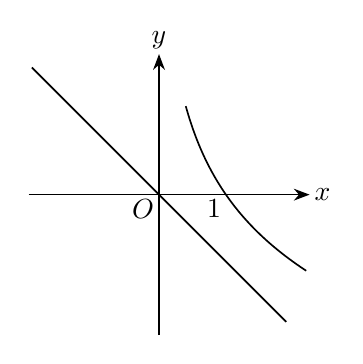
\begin{tikzpicture}[x=0.85cm,y=0.85cm,line width=.6pt,>=Stealth,font=\normalsize]
\coordinate (O) at (0,0);
\coordinate (Xstart) at (-1.95,0);
\coordinate (Xend) at (2.25,0);
\coordinate (Ystart) at (0,-2.10);
\coordinate (Yend) at (0,2.10);
\coordinate (Ux) at (1,0);
\coordinate (A) at (-1.90,1.90);
\coordinate (B) at (1.90,-1.90);
\draw[->] (Xstart)--(Xend) node[right,inner sep=1.5pt] {$x$};
\draw[->] (Ystart)--(Yend) node[above,inner sep=1.5pt] {$y$};
\draw (A)--(B);
\draw[domain=0.40:2.20,samples=120] plot (\x,{-ln(\x)/ln(2)});
\node[below left,inner sep=1.5pt] at (O) {$O$};
\node[below left,inner sep=1.5pt] at (Ux) {$1$};
\end{tikzpicture}
